% LaTeX2e Template by Stephen Iota (https://stepheniota.github.io/)
% last updated: Oct. 2018

% for papers
%\documentclass[aps,onecolumn,superscriptaddress]{revtex4-1}
% https://www-d0.fnal.gov/Run2Physics/WWW/templates/revtex4.pdf
% https://cdn.journals.aps.org/files/revtex/auguide4-1.pdf
% for revTeX4-1 class options

% for other
\documentclass[12pt]{article}
\usepackage[margin=2cm]{geometry}

%%%%%%%%%%%%%%%%
%%% Packages %%%
%%%%%%%%%%%%%%%%

\usepackage[utf8]{inputenc}
\usepackage{amsmath}
\usepackage{amssymb}
\usepackage{amsfonts} % to remove math font when typesetting equations
\usepackage{graphicx}
\usepackage[shortlabels]{enumitem} % to change labels in enum/item
\usepackage[dvipsnames]{xcolor} % for colored links


% always put this at the end
\usepackage[
	colorlinks=true,
	citecolor=green!50!black,
	linkcolor=NavyBlue!75!black,
	urlcolor=green!50!black,
	hypertexnames=false]{hyperref} 

 
 %%%%%%%%%%%%%%%%%%
 %% New Commands %%
 %%%%%%%%%%%%%%%%%%
 
\newcommand{\email}[1]{\texttt{\href{mailto:#1}{#1}}}

\newcommand{\hint}[1]{\color{Blue}{#1}}
 
%----------------------------------------------------
%%%%%%%%%%%%%%%%%%
%% Front Matter %%
%%%%%%%%%%%%%%%%%%

%\pagenumbering{gobble} % no page numbers
\graphicspath{{figures/}} % set directory for figures
\setcounter{section}{-1} % start with section 0

%%%%%%%%%%%%%
%%% Title %%%
%%%%%%%%%%%%%
\begin{document}

\begin{center}

\Large{\textsc{Worksheet 3}: \textbf{Electric Potential}}

\end{center}

\vspace{.5mm}

%%%%%%%%%%
%% INFO %%
%%%%%%%%%%

\begin{tabular}{rl}
\textsc{SI Leader}:
&
Stephen Iota (\email{siota001@ucr.edu})
\\
\textsc{Course}:
&
Physics 40C (Fall 2018), Dr.~Laura Sales
\\
\textsc{Date}:
&
15 October 2018
\end{tabular}

%%%%%%%%%%%%%%
%% PROBLEMS %%
%%%%%%%%%%%%%%

\subsubsection*{Reminder}
\textit{There are no stupid questions!}

\section{Review}

Which surface has more electric flux? Surface A, Surface B, or equal? Explain why.


\begin{center}
	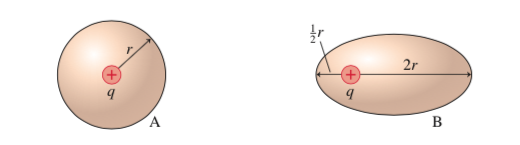
\includegraphics[width=.5\linewidth]{W3-figz}
\end{center}

\vspace{25mm}


\section{Electric Potential}

\begin{enumerate}

\item Is the electric force $\vec{F} = q\vec{E}(\vec{r})$ {\bfseries (a) a conservative force}, {\bfseries (b) a non-conservative force} or {\bfseries (c) a mechanical force}?
\vspace{25mm}
\item How do you determine if a force\footnote{Or similarly, a ``Vector Field.''} is conservative?\footnote{Later in the quarter we will encounter the Lorentz Force which will put these definitions to the test.}
\vspace{10mm}

%%%%% NEW PAGE
\newpage

\item A glass rod is positively charged. The figure below shows the end view of a rod. A negatively charged particle moves in a circular arc around the glass rod. Is the work done on the charged particle by the rod's electric field {\bfseries (a) positive}, {\bfseries(b) negative} or {\bfseries (c) zero}?
\begin{center}
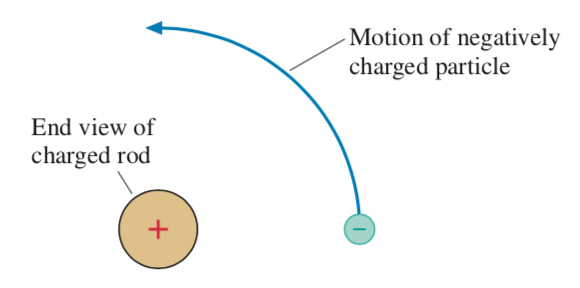
\includegraphics[width=.4\linewidth]{W3-fig1}
\end{center}
\vspace{20mm}
\item Rank in order, from largest to smallest, the potential energies $U_a$ to $U_d$ of these four charge pairs. Each $+$ symbol represents the same amount of charge.
\begin{center}
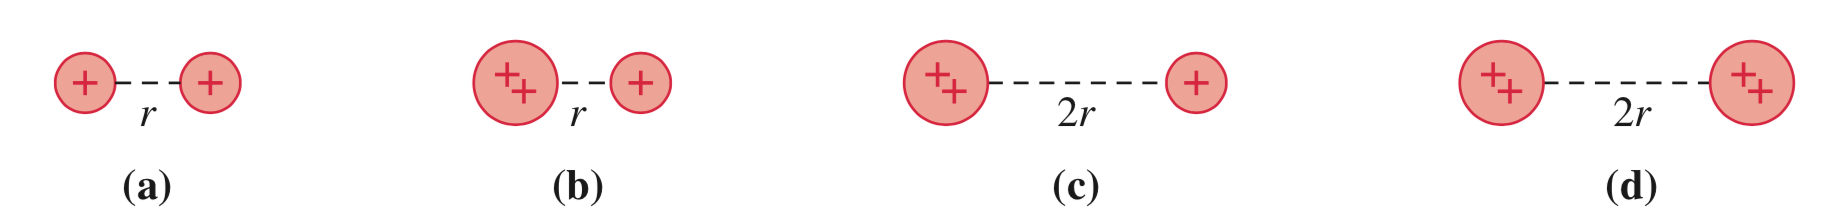
\includegraphics[width=.9\linewidth]{W3-fig2}
\end{center}
\vspace{20mm}


\item A proton is released from rest at point B, where the potential is $0$ V. Afterward, the proton
	\begin{enumerate}[(a)]
	\item Remains at rest at B.
	\item Moves toward A with a steady speed.
	\item Moves toward A with an increasing.
	\item Moves toward C with a steady speed.
	\item Moves toward C with an increasing speed.
	\end{enumerate}

\begin{center}
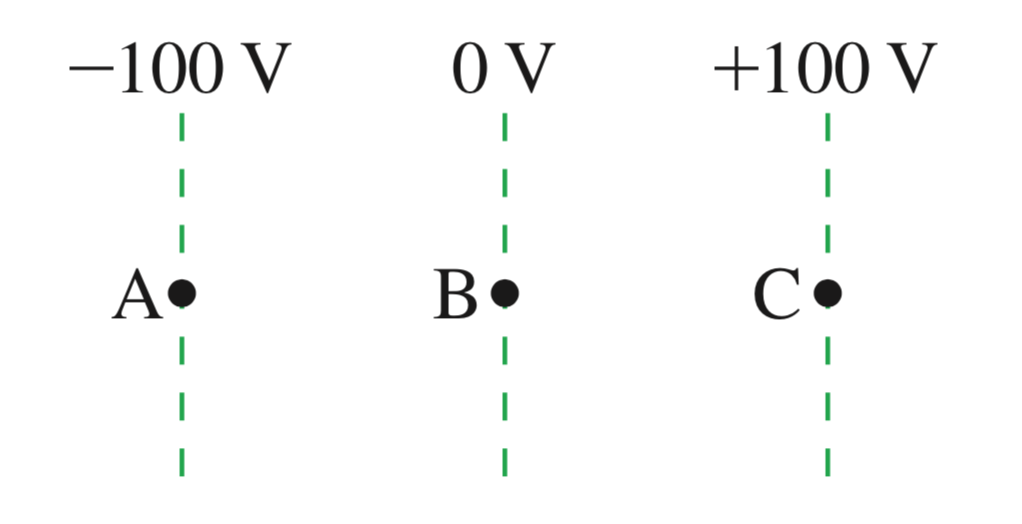
\includegraphics[width=.45\linewidth]{W3-fig3}
\end{center}

\end{enumerate}




\end{document}